%!tex root = ../main.tex
%% Background
%%
\section{Background}
\todo{Could also be named as "Theoretical background"}.
To understand the implementation chapter \ref{sec:solution}, in this section we introduce relevant terminology and concepts.

\todo{Add info about section \ref{sec:graphs}}

In the first section (\ref{sec:distributed_computing}) of this chapter, we discuss about the essential concepts in the theory of distributed computing.
The section aims to explain the meaning of distributed computing and gives an introduction to the main model of distributed computing, \emph{message passing model}, from which many of the researched models inherit from.

The second and third sections discuss about the Port number model and local model respectively.
These are widely used models in the field and they are strongly related to the research showed in this paper.

We are trying to find lower bound proofs for LCL-problems in this paper, therefore it is essential to include a section entirely for them.
The fourth section (\ref{sec:lcl_problems}) is dedicated to LCL-problems.

Finally, in the last section (\ref{sec:previous_research}), we talk about previous research in the field and research that are more related to this thesis.

\subsection{Graphs} \label{sec:graphs}
In the real world, there are many objects that are somehow related to each other can be visualized by a diagrams that consists of points and lines that connect a pair of points.
A graph is a mathematical concept that abstracts the relations of these objects.
In the literature, the points are called vertices and lines are called edges.
\cite{DBLP:books/others/BondyM76}

Mathematically, graph can be defined as a tuple $$G = (V, E)$$ where $V$ is the set of vertices and $E$ is the set of edges.
%Each vertex $v \in V$
Each edge $e \in E$ can also be thought as a tuple $e=(v, w), v, w \in V$, where vertices $v$ and $w$ are the endpoints of the edge $e$.

When the order of the vertices in an edge matters, we call the graph as a \emph{directed graph} or as the shortened variation \emph{digraph}.
For digraphs, the following statement must hold:
\begin{equation} \label{eq:1}
\forall v, w \in V, v \neq w: (v, w) \neq (w, v)
\end{equation}
In that case, the first vertex $v$ points to the vertex $w$.
Usually the edge is visualized as an arrow pointing from $v$ to $w$.
One example of a directed graph is a flow graph, in which the edges represent flows from point to another point, as seen in the figure \ref{fig:graph2}.
An edge of a digraph can also point both directions, but in the example of flow graphs, this does not make sense therefore it is not allowed.

\begin{figure}[h]
  \subcaptionbox{A simple directed graph.}%
    [.3\linewidth] {
    \centering
    \begin{tikzpicture}[>={Latex[length=3mm]},auto, on grid, ]
      \node[main node] (1) {$1$};
      \node[main node] (2) [above right = 1.3cm and 1.5cm of 1] {$2$};
      \node[main node] (3) [below right = 1.3cm and 1.5cm of 1] {$3$};
      \draw[->] (1) edge[] node {} (2);
      \draw[->] (1) edge[] node {} (3);
      \draw[<->] (2) edge[] node {} (3);
    \end{tikzpicture}
    \label{fig:graphs1:a}
  }
  \hfill
  \subcaptionbox{A simple undirected graph.}%
    [.3\linewidth] {
    \centering
    \begin{tikzpicture}[auto, on grid, ]
      \node[main node] (1) {$1$};
      \node[main node] (2) [above right = 1.3cm and 1.5cm of 1] {$2$};
      \node[main node] (3) [below right = 1.3cm and 1.5cm of 1] {$3$};
      \draw[-] (1) edge[] node {} (2);
      \draw[-] (1) edge[] node {} (3);
      \draw[-] (2) edge[] node {} (3);
    \end{tikzpicture}
    \label{fig:graphs1:b}
  }
  \hfill
  \subcaptionbox{An undirected multigraph.}%
    [.3\linewidth] {
    \centering
    \begin{tikzpicture}[auto, on grid, ]
      \node[main node] (1) {$1$};
      \node[main node] (2) [above right = 1.3cm and 1.5cm of 1] {$2$};
      \node[main node] (3) [below right = 1.3cm and 1.5cm of 1] {$3$};
      \draw[-] (1) edge[] node {} (2);
      \draw[-] (1) edge[bend left] node {} (3);
      \draw[-] (1) edge[bend right] node {} (3);
      \draw[-] (2) edge[] node {} (3);
    \end{tikzpicture}
    \label{fig:graphs1:c}
  }
  \caption{Examples of different graphs}
  \label{fig:graphs1}
\end{figure}

\todo{refer the figures from the text and fix old refers}

Undirected graph is the opposite of directed graph in the sense that the order of the vertices in an edge does not matter:
\begin{equation}
\forall v, w \in V: (v, w) = (w, v)
\end{equation}
For the purpose of this work, we need only undirected edges.

The definitions of graphs shown earlier do not restrict an edge to start and end in itself ($e=(v, v)$).
This kind of an edge is called a \emph{loop}.
The definition however restricts multiple same edges, \emph{parallel edges}.
The edge set has to be defined as a multiset in order to allow parallel edges.
A graph that allows parallel edges, is called a \emph{multigraph}.
Depending on the author, multigraphs either allow or disallow loops.
In this work, we consider multigraphs to exist without loops.

A graph that has no loops or parallel edges, is called as a \emph{simple graph}.
Simple graphs can either be directed or undirected and it should be explicitly mentioned when defining graphs, unless the context implies it.






\subsection{Distributed computing} \label{sec:distributed_computing}
Computing or processing a computer program in several identical or different computation nodes is called distributed computing.
It is similiar to running a computer program that contains multiple concurrent tasks, but in distributed computing there are higher level tasks that are distributed to different computer nodes.

Computation nodes are connected to each others with communication channels.
These communication channels carry data from node to another node.
Together, nodes and communication channels form a network.
The best way to visualize these networks is by drawing a graph in which the nodes represent computing nodes and edges represent the communication channels.

\begin{figure}[h]
  \centering
  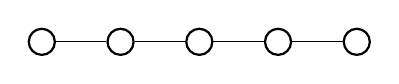
\begin{tikzpicture}[every node/.style={circle,thick,draw}]
  \node (1) {};
  \node (2) [ right of=1] {};
  \node (3) [ right of=2] {};
  \node (4) [ right of=3] {};
  \node (5) [ right of=4] {};
  \draw (1) -- (2);
  \draw (2) -- (3);
  \draw (3) -- (4);
  \draw (4) -- (5);
\end{tikzpicture}
\caption{Example of a distributed network.}
\label{fig:graph1}
\end{figure}

According to Lamport \cite{DBLP:books/el/leeuwen90/LamportL90}, in the area of distributed computing, the term \emph{model} denotes a view or abstract representation of a distributed system.
There are multiple different computation models used in distributed computing.
The most important main category of distributed computation models is \emph{process models}.
In process models, the work or activities are represented as concurrently executed processes that execute their instructions sequentially.
The main way to distinguish different process models from each other is to categorise them by the method they use to communicate with each other (\emph{interprocess communication}).
\cite{DBLP:books/el/leeuwen90/LamportL90}

Message passing models are a form of process model.
They are widely researched, for example ... \todo{add references to papers that research or use message passing models}
In the model, processes communicate by adding a message to message queue, wheter it is a shared or a process specific, and the recipient process removes the message (dequeues) from the message queue.
\cite{DBLP:books/el/leeuwen90/LamportL90}


%The following two sections (\ref{sec:port_number_model} and \ref{sec:local_model} ) talk about different forms of message passing models that are highly relative to this paper.

%In the theory of distributed computing, it is common to use terminology and concepts from graph theory as networks are basically graphs.
%With formal definitions, we can discuss more about the structure of distributed networks and reason features of those networks.
%We can further construct proofs of different theorems and so on. \todo{Fix this paragraph}

The algorithms that are executed in distributed fashion, are called distributed algorithms. \todo{where to write about distributed algorithms?}
%A distributed algorithm is a specific type of algorithm that is executed in distributed fashion.
Specifically, each node executes the same algorithm.

\todo{write about computation models, why they exist}
\todo{Add message passing model before PN model}
\subsubsection{Message passing model} \label{sec:message_passing_model}
\subsubsection{Port Number model} \label{sec:port_number_model}
\subsubsection{LOCAL model} \label{sec:local_model}
\subsection{LCL problems} \label{sec:lcl_problems}
\subsection{Previous research} \label{sec:previous_research}
\todo{Especially LCL classification research}
\clearpage
